\documentclass[%
	%final, %
	%notes=show,
	% draft, % Grafische Elemente durch graue Boxen ersetzen (beschleunigt Kompilieren)
	% 8pt, % Zu klein, erfordert Paket extsize
	% 9pt, % Zu klein, erfordert Paket extsize
	% 10pt, % für Folien mit sehr viel Text
	11pt, % Standardschriftgröße
	% 12pt, % etwas größer und daher besser zu lesen
	% 14pt, % deutlich größer, erfordert Paket extsize
	% 17pt, % PowerPoint Standardschriftgröße, erfordert Paket extsize
	% 20pt, % sehr groß, erfordert Paket extsize
	% trans,% Zum Erstellen von Overhead Folien
	%handout, % Erstellen eines Handouts
	% article,% Erstellen eines Artikels
 	% compress, % Die Navigation in der Kopfzeile wird komprimiert dargestellt
	%t, % Place text of slides at the (vertical) top of the slides
	% c, % Place text of slides at the (vertical) center of the slides
	% color={}, % list of options for color
	 xcolor={table,dvipsnames}, % Optionen für xcolor übergeben
	 hyperref={}, % list of options for hyperref
	% envcountsect, % Causes theorems, definitions, and so on to be numbered locally to each section.
	% notheorems, % Switches off the definition of default blocks like theorem
	% noamsthm, % Does not load amsthm and also not amsmath
	% ucs, % lädt ucs Paket
	% utf8, % lädt utf8x Paket von ucs (utf8 enconding)
	% dvips, % erzwingt das Laden des dvips Treibers - idR nicht nötig!
	% usepdftitle=false, % Suppresses the automatic generation of title and author entries in the pdf document information.
	% ignorenonframetext, % suppresses content created for the article mode ??
	%show notes, % enables Notes
	% leqno,
	% fleqn,
]{beamer}[2007/03/11] % Minimum necessary version due to severe bugs in version 3.06 !!!

%\setbeameroptions{show notes}

% Folien f�r Druck
%\usepackage{pgfpages}
%\pgfpagesuselayout{resize to}[a4paper,border shrink=5mm,landscape]
%\pgfpagesuselayout{2 on 1}[a4paper,border shrink=5mm]
%
%\pgfpagesuselayout{4 on 1}[a4paper,border shrink=5mm,landscape]
%\pgfpagesuselayout{8 on 1}[a4paper,border shrink=5mm]
%\pgfpagesuselayout{16 on 1}[a4paper,border shrink=5mm,landscape]

% ~~~~~~~~~~~~~~~~~~~~~~~~~~~~~~~~~~~~~~~~~~~~~~~~~~~~~~~~~~~~~~~~~~~~~~~~
% Fonts Fonts Fonts
% ~~~~~~~~~~~~~~~~~~~~~~~~~~~~~~~~~~~~~~~~~~~~~~~~~~~~~~~~~~~~~~~~~~~~~~~~
%\usepackage[T1]{fontenc} % T1 Schrift Encoding
\usepackage{textcomp}	 % additional symbols (Text Companion font extension)


% \usepackage{lmodern}               %% --- Latin Modern
%\usepackage{mathptmx}              %% --- Times mit Matheschriften
% \usepackage{mathpazo}              %% --- Palantino
% \usepackage{charter}               %% --- Charter
% \usepackage{bookman}               %% Bookman (lädt Avant Garde !!)
% \usepackage{newcent}               %% New Century Schoolbook (lädt Avant Garde !!)

% \usepackage{bera}
%\usepackage[scaled=.90]{helvet}    %% --- Helvetica (Arial)
% \usepackage{cmbright}              %% --- CM-Bright (eigntlich eine Familie)
% \usepackage{tpslifonts}            %% --- (Font for Slides)
% \usepackage{avant}      	          %% --- Avantgard
%
%\usepackage{courier}               %% --- Courier
%\usepackage[scaled=0.9]{luximono}  	 %% --- Luxi Mono


%%% ===== Sans Serif (kommerzielle Schriften) ============================

% \usepackage[scaled=0.90]{frutiger}  %% --- Adobe Frutiger
% \usepackage[scaled=0.94]{futura}    %% --- Adobe Futura (=Linotype FuturaLT) : Sans Serif
% \usepackage{gillsans}               %% --- Adobe Gill Sans : Sans Serif
% \renewcommand{\sfdefault}{pmy}      %% -- Adobe Myriad  : Sans Serif
% \usepackage[scaled]{asyntax}        %% --- Syntax : sans serif font
% \usepackage[medium]{optima}         %% --- Adobe Optima : Semi Sans Serif
% \renewcommand{\sfdefault}{lo9}      %% --- Linotype ITC Officina Sans

%% ===== Serifen (kommerzielle Schriften ) ================================

% \renewcommand{\rmdefault}{pasx}     %% --- Adobe Aldus
% \usepackage[scaled=1.05]{xagaramon} %% --- Adobe Garamond
% \renewcommand{\rmdefault}{pegx}     %% --- Adobe Stempel Garamond
% \renewcommand{\rmdefault}{pml}      %% --- Adobe Melior
% \renewcommand{\rmdefault}{pmnx}     %% --- Adobe Minion
% \renewcommand{\rmdefault}{psbx}     %% --- Adobe Sabon
% \renewcommand{\rmdefault}{lch}      %% --- Linotype ITC Charter
% \renewcommand{\rmdefault}{lmd}      %% --- Linotype Meridien
\usefonttheme[onlymath]{serif}
% *** Sprache *****************************
\usepackage[ngerman]{babel}
\usepackage[applemac]{inputenc}
%------------------------------------------


%%% Doc: ftp://tug.ctan.org/pub/tex-archive/macros/latex/required/graphics/grfguide.pdf
% Bilder
\usepackage[%
   %final,
   %draft % do not include images (faster)
]{graphicx}



%%% Emulationspakete
% \usepackage{beamerprosper}
% \usepackage{beamerseminar}
% \usepackage{beamerfoils}
% \usepackage{beamertexpower}


%%% 4.6.2    Printing the Handout
% \usepackage{pgfpages}
% \pgfpagelayout{resize}[a4paper,border shrink=5mm,landscape]
%     This says “Resize all pages to landscape A4 pages, no what their original size was, but shrink the pages
% by 5mm, so that there is a bit of a border around everything.” Naturally, instead of a4paper you can also use
% letterpaper or any of the other standard paper sizes. For further options and details see the documentation
% of pgfpages.
% \pgfpagelayout{2 on 1}[a4paper,border shrink=5mm]


% \usepackage{multimedia}
%     A stand-alone package that implements several commands for including external animation and sound
%     files in a pdf document. The package can be used together with both dvips plus ps2pdf and pdflatex,
%     though the special sound support is available only in pdflatex.



%% sonstige Pakete ========================
%
% \usepackage{enumitem}
% \usepackage{units}
% \usepackage{pifont}
% \usepackage{subscript}
% -----------------------------------------

\usepackage{tabularx}   % Erweiterte Tabellen Optionen
\usepackage{booktabs}
\usepackage{multicol}
\usepackage{units}
\usepackage{nicefrac}

\usepackage[T1]{fontenc} %Schriftarten laden
\usepackage[T1]{pbsi}
\newcommand{\changefont}[3]{
\fontfamily{#1} \fontseries{#2} \fontshape{#3} \selectfont}

\usepackage{oldgerm}
\usepackage{pifont}

\usepackage{/Users/waj/Documents/Mathematik/mymath}
\usepackage{pgf,tikz}
\usetikzlibrary{arrows}
\usetikzlibrary{positioning}
\usetikzlibrary{shadows}

\usepackage{multimedia}

\usepackage{geometry}
\usepackage{graphicx}

\usepackage{framed}
\usepackage{tikz-er2}


% *****************************************
% >>> Themes <<<<<<<<<<<<<<<<<<<<<<<<<<<<<<
% *****************************************

% \usetheme[<options>]{<name list>} 		Installs the presentation theme named <name>.
% \usecolortheme[<options>]{<name list>} Same as \usetheme, only for color themes.
% \usefonttheme[<options>]{<name>} 		Same as \usetheme, only for font themes.
% \useinnertheme[<options>]{<name>}		Same as \usetheme, only for inner themes.
% \useoutertheme[<options>]{<name>}		Same as \usetheme, only for outer themes.

% *****************************************
% >>> Themes ohne Navigation
% *****************************************
% \usetheme{default}
% -------------------------------
% \usetheme[]{Bergen}
% -------------------------------
% \usetheme[%
% 	secheader % section im Header
% ]{Boadilla}
% -------------------------------
% % Wie das Boadilla theme, mit kraeftigeren Farben
% % und unveraenderten Icons
% \usetheme[%
% 	secheader % section im Header
% ]{Madrid}
% -------------------------------
% \usetheme{Pittsburgh}
% -------------------------------
% \usetheme[]{Rochester}


% *****************************************
% >>> Themes mit Navigation (Baumstruktur)
% *****************************************
% \usetheme{Antibes}      % flach
% -------------------------------
% \usetheme{JuanLesPins}  % 3D, Schatten
% -------------------------------
% \usetheme{Montpellier}    % flach, wenig Farben


% *****************************************
% >>> Themes mit Navigation (Sidebar)
% *****************************************
% % flach, starke Farben
% \usetheme[%
%  	left, % sidebar links
% % 	right, % sidebar rechts
% % 	hideallsubsections, % nur sections werden angezeigt
% % 	hideothersubsections, % nur subsections der aktuellen section werden angezeigt
% ]{Berkeley}
% -------------------------------
% % wie Berkeley, 3D, starke Farben
% \usetheme[%
%  	left, % sidebar links
% % 	right, % sidebar rechts
% % 	hideallsubsections, % nur sections werden angezeigt
% % 	hideothersubsections, % nur subsections der aktuellen section werden angezeigt
% ]{PaloAlto}
% -------------------------------
% % flach, schwache Farben
% \usetheme[%
%  	left, % sidebar links
% % 	right, % sidebar rechts
% % 	hideallsubsections, % nur sections werden angezeigt
% % 	hideothersubsections, % nur subsections der aktuellen section werden angezeigt
% ]{Goettingen}
% -------------------------------
% % wie Goettingen, flach, starke Farben
% \usetheme[%
%  	left, % sidebar links
% % 	right, % sidebar rechts
% % 	hideallsubsections, % nur sections werden angezeigt
% % 	hideothersubsections, % nur subsections der aktuellen section werden angezeigt
% ]{Marburg}
% -------------------------------
% flach, schwache Farben
% \usetheme[%
% % 	hideallsubsections, % nur sections werden angezeigt
% % 	hideothersubsections, % nur subsections der aktuellen section werden angezeigt
% ]{Hannover}


% *****************************************
% >>> Themes mit Navigation (Mini Frame Navigation)
% *****************************************
% % starke Farben, flach
% \usetheme[
% % 	compress, % Navigation in einer Zeile
% ]{Berlin}
% -------------------------------
% % wie Berlin, runde Kanten, starke Farben, flach
% \usetheme[
% 	compress, % Navigation in einer Zeile
% ]{Ilmenau}
% -------------------------------
% % wie Berlin, starke Farben, flach
% \usetheme[
% 	compress, % Navigation in einer Zeile
% ]{Dresden}
% -------------------------------
% % starke Farben, 3D
% \usetheme{Darmstadt}
% -------------------------------
% % wie Darmstadt, ohne subsections
% \usetheme{Frankfurt}
% -------------------------------
% % flach, schwache Farben
% \usetheme{Singapore}
% -------------------------------
% % flach, horiz. Linien
% \usetheme{Szeged}


% *****************************************
% >>> Themes mit Navigation (Section and Subsection Tables)
% *****************************************
% % flach, rund, starke Farben
% \usetheme{Copenhagen}
% -------------------------------
% % flach, eckig, starke Farben
% \usetheme{Luebeck}
% -------------------------------
% % flach, starke Farben
% \usetheme{Malmoe}
% -------------------------------
% 3D, starke Farben
\usetheme{Warsaw}


% *****************************************
% >>>> 15.1    Inner Themes
% *****************************************
% An inner theme installs templates that dictate how the following elements are typeset:
%    - Title and part pages.
%    - Itemize environments.
%    - Enumerate environments.
%    - Description environments.
%    - Block environments.
%    - Theorem and proof environments.
%    - Figures and tables.
%    - Footnotes.
%    - Bibliography entries.


% >>>  Itemize Bullets
% -------------------------------
% \useinnertheme{default} % Zahlen
% -------------------------------
% \useinnertheme{circles} % Kreise
% -------------------------------
%\useinnertheme{rectangles} % Vierecke
% -------------------------------
% \useinnertheme[%
 %	shadow % mit Schatten
 %]{rounded} % 3D Kugeln
% -------------------------------
% \useinnertheme{inmargin} % Bullts im Margin


% *****************************************
% >>>> 15.2    Outer Themes
% *****************************************
% An outer theme dictates (roughly) the overall layout of frames. It specifies where any navigational elements
% should go (like a mini table of contents or navigational mini frames) and what they should look like. Typically,
% an outer theme specifies how the following elements are rendered:
%    - The head- and footline.
%    - The sidebars.
%    - The logo.
%    - The frame title.

% \useoutertheme{default}
% -------------------------------
% \useoutertheme{infolines}
% -------------------------------
% \useoutertheme[%
% 	footline=empty, % suppressed the footline (default).
% % 	footline=authorinstitute, %shows the author's name and the institute in the footline.
% % 	footline=authortitle, % shows the author's name and the title in the footline.
% % 	footline=institutetitle, % shows the institute and the title in the footline.
% % 	footline=authorinstitutetitle, % shows the author's name, the institute, and the title in the footline.

% ]{miniframes}
% -------------------------------
% \useoutertheme[%
% % 	subsection= true,  % or false shows or suppresses line showing the subsection in the headline.
% ]{smoothbars}
% -------------------------------
% \useoutertheme[%
%  	left, % sidebar links
% % 	right, % sidebar rechts
% % 	hideallsubsections, % nur sections werden angezeigt
% % 	hideothersubsections, % nur subsections der aktuellen section werden angezeigt
% ]{sidebar}
% -------------------------------
% % This theme installs a headline in which, on the left, the sections of the talk are shown and, on the right,
% % the subsections of the current section. If the class option compress has been given, the sections and
% % subsections will be put in one line; normally there is one line per section or subsection.
% \useoutertheme{split}
% The colors are taken from palette primary and palette fourth.
% -------------------------------
% % This layout theme extends the split theme by putting a horizontal shading behind the frame title and
% % adding a little 'shadow' at the bottom of the headline.
% \useoutertheme{shadow}
% -------------------------------
% \useoutertheme[
% % 	hooks, % Einruecken der Abschnittsueberschriften in der Kopfzeile
% ]{tree}
% -------------------------------
% wie tree, ohne die Linien
% \useoutertheme{smoothtree}


% *****************************************
% >>>> 16.1    Color Themes
% *****************************************
% \usecolortheme{default}
% \usecolortheme{structure}
% \usecolortheme{sidebartab}

% *****************************************
% >>>> 16.1.2    Complete Color Themes
% A 'complete' color theme is a color theme that completely specifies all colors for all parts of a frame. It
% installs specific colors and does not derive the colors from, say, the structure beamer-color. Complete
% color themes happen to have names of flying animals.

% -------------------------------
% \usecolortheme{default}
% -------------------------------
\usecolortheme[%
% 	named=red,
 	named=blue,
% 	named=green,
% 	named=orange,
% 	named=gray,
% 	named=NavyBlue,
%  named=RoyalBlue,
%  named=MidnightBlue,
%  named=CadetBlue,
]{structure}
% Farben aus dvipsnam.def: (Option 'dvipsnames' fuer xcolor muss geladen sein!)
% http://www.math.utu.fi/opetusohj/latex/doc/palette.pdf
% GreenYellow, Yellow, Goldenrod, Dandelion, Apricot, Peach, Melon, YellowOrange, Orange, BurntOrange, Bittersweet, RedOrange, Mahogany, Maroon, BrickRed, Red, OrangeRed, RubineRed, WildStrawberry, Salmon, CarnationPink, Magenta, VioletRed, Rhodamine, Mulberry, RedViolet, Fuchsia, Lavender, , Thistle, Orchid, DarkOrchid, Purple, Plum, Violet, RoyalPurple, BlueViolet, Periwinkle, CadetBlue, CornflowerBlue, MidnightBlue, NavyBlue, RoyalBlue, Blue, Cerulean, Cyan, ProcessBlue, , SkyBlue, Turquoise, TealBlue, Aquamarine, BlueGreen, Emerald, JungleGreen, SeaGreen, Greenv,  ForestGreen, PineGreen, LimeGreen, YellowGreen, SpringGreen, OliveGreen, RawSienna, Sepia, Brown, Tan, Gray, Black, White
% -------------------------------
% % blau-schwarz, Hintergrund: blau
% \usecolortheme[%
% %  	overlystylish
% ]{albatross}
% -------------------------------
% % blau-schwarz, Hintergrund: weiss
% \usecolortheme{lily}
% -------------------------------
% % blau-grau, , Hintergrund: grau
% \usecolortheme{beetle}
% -------------------------------
% % gelb-weiss, , Hintergrund: weiss
% \usecolortheme{crane}
% -------------------------------
% grau-grau (hell)
% \usecolortheme{dove}
% -------------------------------
% % grau-grau (dunkel)
% \usecolortheme{fly}
% -------------------------------
% % grau-grau-weiss (hell) mit Boxen
% \usecolortheme{seagull}
% -------------------------------
% % gelb-orange-grau
% \usecolortheme{wolverine}
% -------------------------------
% % grau
% \usecolortheme{beaver}

% *****************************************
% >>>> 16.1.3    Inner Color Themes
% Inner color themes only specify the colors of elements used in inner themes. Most noticably, they specify
% the colors used for blocks. They can be used together with other (color) themes. If they are used to change
% the inner colors installed by a presentation theme or another color theme, they should obviously be specified
% after the other theme has been loaded. Inner color themes happen to have fl�ower names.
% -------------------------------
% \usecolortheme{lily} % keine Boxen
% -------------------------------
% \usecolortheme{orchid} % Boxen mit starken Farben
% -------------------------------
% \usecolortheme{rose} % Boxen mit schwachen Farben

% *****************************************
% >>>> 16.1.4    Outer Color Themes
% An outer color theme changes the palette colors, on which the colors used in the headline, footline, and
% sidebar are based by default. Outer color themes normally do not change the color of inner elements, except
% possibly for titlelike. They have happen to sea-animal names.

% -------------------------------
% % Titel mit Farbe, starke Farben
% \usecolortheme{whale}
% -------------------------------
% % Titel mit Farbe, schwache Farben
% \usecolortheme{seahorse}
% -------------------------------
% % Titel ohne Farbe, starke Farben
% \usecolortheme{dolphin}

% *****************************************
% Detailierte Veraenderungen der Farben
% *****************************************
% \setbeamercolor*{author in head/foot}{parent=palette tertiary}
% \setbeamercolor*{title in head/foot}{parent=palette secondary}
% \setbeamercolor*{date in head/foot}{parent=palette primary}
% \setbeamercolor*{section in head/foot}{parent=palette secondary} %tertiary
% \setbeamercolor*{subsection in head/foot}{parent=palette primary}
% Elemente deren Farbe veraendert werden kann
% \setbeamercolor{normal text}{fg=black}
% \setbeamercolor*{example text}
% \setbeamercolor*{titlelike}
% \setbeamercolor*{separation line}
% \setbeamercolor*{upper separation line head}
% \setbeamercolor*{separation line}
% \setbeamercolor*{middle separation line head}
% \setbeamercolor*{separation line}
% \setbeamercolor*{lower separation line head}
% \setbeamercolor*{upper separation line foot}
% \setbeamercolor*{middle separation line foot}
% \setbeamercolor*{lower separation line foot}
% -------------------------------
% \setbeamercolor*{math text}
% \setbeamercolor*{math text inlined}
% \setbeamercolor*{math text displayed}
% \setbeamercolor*{normal text in math text}
% -------------------------------
% Nutzung:
% \usebeamercolor[fg]{normal text}
% \setbeamercolor{normal text}{fg=black,bg=mylightgrey}
% -------------------------------
% Palette:
% \setbeamercolor{palette primary}
% \setbeamercolor{palette secondary}
% \setbeamercolor{palette tertiary}
% \setbeamercolor{palette quaternary}
% -------------------------------
% \setbeamercolor{palette sidebar primary}
% \setbeamercolor{palette sidebar secondary}
% \setbeamercolor{palette sidebar tertiary}
% \setbeamercolor{palette sidebar quaternary}




% *****************************************
% Transparenz Effekte
% *****************************************

\setbeamercovered{invisible} % is the default and causes covered text to 'completely disappear.
% \setbeamercovered{transparent} % Durchscheinen des Textes
% \setbeamercovered{dynamic} % Einblenden
% \setbeamercovered{highly dynamic} % Einblenden


% *****************************************
% >>>> 17.1 Font Themes
% *****************************************
% \usefonttheme{default}
% The default font theme installs a sans serif font for all text of the presentation. The default theme
% installs different font sizes for things like titles or head- and footlines, but does not use boldface or
% italics for 'hilighting.' To change some or all text to a serif font, use the serif theme.
% -------------------------------
% \usefonttheme{professionalfonts}
% This font theme does not really change any fonts. Rather, it suppresses certain internal replacements
% performed by beamer. If you use 'professional fonts' (fonts that you buy and that come with a
% complete set of every symbol in all modes), you do not want beamer to meddle with the fonts you use.
% -------------------------------
% \usefonttheme[%
% % 	stillsansserifmath, % mathematical text typeset using sans serif.
% % 	stillsansserifsmall, % will cause 'small' text to be still typeset using sans serif. This refers to
%  								% the text in the headline, footline, and sidebars. Using this options is often
%  								% advisable since small  text is often easier to read in sans serif.
% % 	stillsansseriflarge, %  Titel still   typeset using sans serif
% %  	onlymath, % typset math in serif but nothing else
% ]{serif}
% -------------------------------
% \usefonttheme[%
% % 	onlysmall, % headline, footline, and sidebars is changed
% % 	onlylarge, % main title, frame titles, and section
% ]{structurebold}
% -------------------------------
% \usefonttheme[%
% % 	onlysmall, % headline, footline, and sidebars is changed
% % 	onlylarge, % main title, frame titles, and section
% ]{structureitalicserif}
% -------------------------------
% \usefonttheme[%
% % 	onlysmall, % headline, footline, and sidebars is changed
% % 	onlylarge, % main title, frame titles, and section
% ]{structuresmallcapsserif}



% *****************************************
% >>>> Veraendern der Schrifteinstellung definierter Elemente
% *****************************************

% Beispiele
% \setbeamerfont{frametitle}{size=\large}
% \setbeamerfont{frametitle}{series=\bfseries}

% weitere Befehle
% size= size command sets the size attribute of the beamerfont.
% size*={ size in pt }{ baselineskip }
% shape= (\itshape, \slshape, \scshape, or \upshape)
% series= (command like \bfseries.)
% family= (command like \rmfamily or \sffamily).
% family*={ family name } (For example, the family name for Times happens to be ptm. )
% parent={ parent list } specifies a list of parent fonts.
%
% Example for parent
% \setbeamerfont{parent A}{size=\large}
% \setbeamerfont{parent B}{series=\bfseries}
% \setbeamerfont{child}{parent={parent A, parent B},size=\small}
%
% \usebeamerfont{child}
% This text is small and bold.

% *****************************************
% >>>> 15.3.2    Using Beamer's Templates
% *****************************************
% As a user of the beamer class you typically do not 'use' or 'invoke' templates yourself, directly. For
% example, the frame title template is automatically invoked by beamer somewhere deep inside the frame
% typesetting process. The same is true of most other templates. However, if, for whatever reason, you wish
% to invoke a template yourself, you can use the following command.
% \usebeamertemplate***{ element name }
% -------------------------------
%%% 7.2.1 The Headline and Footline
% \setbeamertemplate{headline} % Beamer-Template/-Color/-Font
% \setbeamertemplate{headline}
% {%
%   \begin{beamercolorbox}{section in head/foot}
%     \vskip2pt\insertnavigation{\paperwidth}\vskip2pt
%   \end{beamercolorbox}%
% }
% \setbeamertemplate{headline}[default] % The default is just an empty headline.
% \setbeamertemplate{headline}[infolines theme]
% \setbeamertemplate{headline}[miniframes theme]
% \setbeamertemplate{headline}[sidebar theme]
% \setbeamertemplate{headline}[smoothtree theme]
% \setbeamertemplate{headline}[smoothbars theme]
% \setbeamertemplate{headline}[tree]
% \setbeamertemplate{headline}[split theme]
% \setbeamertemplate{headline}[text line]{ text } % The headline is typeset with 'text'
% -------------------------------
% \setbeamertemplate{footline} % Beamer-Template/-Color/-Font
% \setbeamertemplate{footline}[default]
% \setbeamertemplate{footline}[infolines theme]
% \setbeamertemplate{footline}[miniframes theme]
% \setbeamertemplate{footline}[page number]
% \setbeamertemplate{footline}[frame number]
% \setbeamertemplate{footline}[split]
% \setbeamertemplate{footline}[text line]{ text }
% -------------------------------
%%% 7.2.2 The Sidebars
% -------------------------------
%%% 7.2.3 Navigation Bars (funktioniert nur mit miniframe Themes)
% \setbeamertemplate{mini frames}[default] % shows small circles as mini frames.
\setbeamertemplate{mini frames}[box] % shows small rectangles as mini frames.
% \setbeamertemplate{mini frames}[tick] % shows small vertical bars as mini frames.
% -------------------------------
%%% 7.2.4 The Navigation Symbols
%%% Beamer-Template/-Color/-Font navigation symbols
\setbeamertemplate{navigation symbols}{} % suppresses all navigation symbols:
% \setbeamertemplate{navigation symbols}[horizontal] % Organizes the navigation symbols horizontally.
% \setbeamertemplate{navigation symbols}[vertical] % Organizes the navigation symbols vertically.
% \setbeamertemplate{navigation symbols}[only frame symbol] % Shows only the navigational symbol for navigating frames.
% -------------------------------
%%% 7.2.5 The Logo
% \setbeamertemplate{logo} % Beamer-Template/-Color/-Font
% -------------------------------
%%% 7.2.6 The Frame Title
% \setbeamertemplate{frametitle} % Beamer-Template/-Color/-Font
% \setbeamertemplate{frametitle}[default][left] % left, center, right
% \setbeamertemplate{frametitle}[shadow theme]
% \setbeamertemplate{frametitle}[sidebar theme]
% \setbeamertemplate{frametitle}[smoothbars theme]
% \setbeamertemplate{frametitle}[smoothtree theme]
% -------------------------------
%%% 7.2.7 The Background
% \setbeamertemplate{background canvas} % Beamer-Template/-Color/-Font
% \setbeamertemplate{background canvas}[default]
% \setbeamertemplate{background canvas}[vertical shading][ color options ] installs a vertically shaded background.
%     - top= color specifies the color at the top of the page. By default, 25% of the foreground of
%       the beamer-color palette primary is used.
%     - bottom= color specifies the color at the bottom of the page. By default, the background of
%       normal text at the moment of invocation of this command is used.
%     - middle= color specifies the color for the middle of the page. Thus, if this option is given, the
%       shading changes from the bottom color to this color and then to the top color.
%     - midpoint= factor specifies at which point of the page the middle color is used. A factor of 0
%       is the bottom of the page, a factor of 1 is the top. The default, which is 0.5 is in the middle.
% \setbeamertemplate{background} % Beamer-Template/-Color/-Font
% \setbeamertemplate{background}[default] % is empty.
% \setbeamertemplate{background}[grid][step=1cm] % places a grid on the background.
%     - step= dimension specifies the distance between grid lines. The default is 0.5cm.
%     - color= color specifies the color of the grid lines. The default is 10% foreground.
% -------------------------------
%%% 7.3 Margin Sizes
\setbeamersize{text margin left=2em,text margin right=2em}
% \setbeamersize{sidebar width left=2cm}
%         - text margin left= TEX dimension sets a new left margin. This excludes the left sidebar. Thus,
%           it is the distance between the right edge of the left sidebar and the left edge of the text.
%         - text margin right= TEX dimension sets a new right margin.
%         - sidebar width left= TEX dimension sets the size of the left sidebar. Currently, this command
%           should be given before a shading is installed for the sidebar canvas.
%         - sidebar width right= TEX dimension sets the size of the right sidebar.
%         - description width= TEX dimension sets the default width of description labels, see Section 11.1.
%         - description width of= text sets the default width of description labels to the width of the
%             text , see Section 11.1.
%         - mini frame size= TEX dimension sets the size of mini frames in a navigation bar. When two
%           mini frame icons are shown alongside each other, their left end points are TEX dimension far
%           apart.
%         - mini frame offset= TEX dimension set an additional vertical offset that is added to the mini
%           frame size when arranging mini frames vertically.
% -------------------------------
%%% 9.1 Adding a Title Page
% \setbeamersize{title page} % Beamer-Template/-Color/-Font
%    This template is invoked when the \titlepage command is used.
%    The following commands are useful for this template:
%     -  \insertauthor inserts a version of the author's name that is useful for the title page.
%     -  \insertdate inserts the date.
%     -  \insertinstitute inserts the institute.
%     -  \inserttitle inserts a version of the document title that is useful for the title page.
%     -  \insertsubtitle inserts a version of the document title that is useful for the title page.
%     -  \inserttitlegraphic inserts the title graphic into a template.
% -------------------------------
%%% 9.2 Adding Sections and Subsections
% -------------------------------
%%% Parent Beamer-Template sections/subsections in toc
% This is a parent template, whose children are section in toc and subsection in toc.
% \setbeamertemplate{sections/subsections in toc}[default]
% \setbeamertemplate{sections/subsections in toc}[sections numbered]
% \setbeamertemplate{sections/subsections in toc}[subsections numbered]
% \setbeamertemplate{sections/subsections in toc}[circle]
\setbeamertemplate{sections/subsections in toc}[square]
% \setbeamertemplate{sections/subsections in toc}[ball]
% \setbeamertemplate{sections/subsections in toc}[ball unnumbered]
% -------------------------------
%%% 9.6 Adding a Bibliography
% -------------------------------
% \setbeamertemplate{bibliography item} % Beamer-Template/-Color/-Font
\setbeamertemplate{bibliography item}[default] %  little article icon as the reference
% \setbeamertemplate{bibliography item}[article] % Alias for the default.
% \setbeamertemplate{bibliography item}[book] % little book icon as the reference
% \setbeamertemplate{bibliography item}[triangle] % triangle as the reference
% \setbeamertemplate{bibliography item}[text] % reference text (like '[Dijkstra, 1982]')
% -------------------------------
%%% 10.1 Adding Hyperlinks and Buttons
% -------------------------------
%%% 11.1 Itemizations, Enumerations, and Descriptions
% \setbeamertemplate{items} % parent template of itemize items and enumerate items
% \setbeamertemplate{itemize items} % Parent Beamer-Template
% \setbeamertemplate{itemize items}[triangle]
% \setbeamertemplate{itemize items}[circle]
% \setbeamertemplate{itemize items}[square]
% \setbeamertemplate{itemize items}[ball]
% -------------------------------
% \setbeamertemplate{enumerate items}[default] % Numbered
% \setbeamertemplate{enumerate items}[circle] % Places the numbers inside little circles.
% \setbeamertemplate{enumerate items}[square] % Places the numbers on little squares.
 \setbeamertemplate{enumerate items}[ball] % 'Projects' the numbers onto little balls.
% -------------------------------
%%% 11.2 Hilighting
% -------------------------------
%%% 11.3 Block Environments
% \setbeamertemplate{blocks} % Parent Beamer-Template
% \setbeamertemplate{blocks}[default]
\setbeamertemplate{blocks}[rounded][shadow=true]
% \setbeamertemplate{blocks}[rounded][shadow=false]
% -------------------------------
%%% 11.4 Theorem Environments
% \setbeamertemplate{qed symbol} % Beamer-Template/-Color/-Font
% -------------------------------
% \setbeamertemplate{theorems} % Parent Beamer-Template
% \setbeamertemplate{theorems}[default]
% \setbeamertemplate{theorems}[normal font]
% \setbeamertemplate{theorems}[numbered]
% \setbeamertemplate{theorems}[ams style]
% -------------------------------
%%% 11.6 Figures and Tables
% \setbeamertemplate{caption} % Beamer-Template/-Color/-Font
% \setbeamertemplate{caption}[default] typesets the caption name (a word like 'Figure' or 'Abbildung' or 'Table')
% \setbeamertemplate{caption}[numbered] adds the figure or table number to the caption.
% \setbeamertemplate{caption}[caption name own line]
% -------------------------------
% \setbeamertemplate{caption name} % Beamer-Color/-Font
% -------------------------------
%%% 11.10    Abstract
% -------------------------------
%%% 11.11 Verse, Quotations, Quotes
% -------------------------------
%%% 11.12 Footnotes
% -------------------------------
%%% 18.1 Specifying Note Contents
% \setbeamertemplate{note page} % Beamer-Template/-Color/-Font
% \setbeamertemplate{note page}[default]
% \setbeamertemplate{note page}[compress]
% \setbeamertemplate{note page}[plain]
% -------------------------------
%%% Specifying Which Notes and Frames Are Shown
% \setbeameroption{hide notes}
% \setbeameroption{show notes}
% \setbeameroption{show notes on second screen= location }
% \setbeameroption{show only notes}
%% Eigene Definitionen ============================
%

\newcommand{\therfore}{\ding{225}\mbox{ }}
\newcommand{\verythinarrow}{\ding{221}\mbox{ }}
\newcommand{\thinarrow}{\ding{222}\mbox{ }}
\newcommand{\newarrow}{\ding{222}\mbox{ }}
\newcommand{\addspace}{\vspace{0.5\baselineskip}}

% Command, um Tabellen-Spalten anzupassen
\newcommand{\spaltenheight}{\rule{0mm}{3ex}}
\newcommand{\spaltenwidth}{\rule{3cm}{0mm}}
\newcommand{\spaltensep}{\\[1ex]}

% Farben
\definecolor{Gray}{gray}{0.9}
\definecolor{darkgreen}{rgb}{0,0.4,0}
\definecolor{lightyellow}{rgb}{1,1,0.8}
\begin{document}
	\title{Tartaglia und die Gleichung 3. Grades}
\subtitle{\glqq Vom Unl�sbaren zum Unvorstellbaren\grqq}
\author{Jorma Wassmer}
\institute{Gymnasium K�niz-Lerbermatt}
\titlegraphic{}
\date{\today}


\begin{frame}[plain]
  \titlepage
\end{frame}
	\section{Das Duell}

\begin{frame}
\frametitle{Venedig}
\framesubtitle{16. Jahrhundert}

\begin{center}
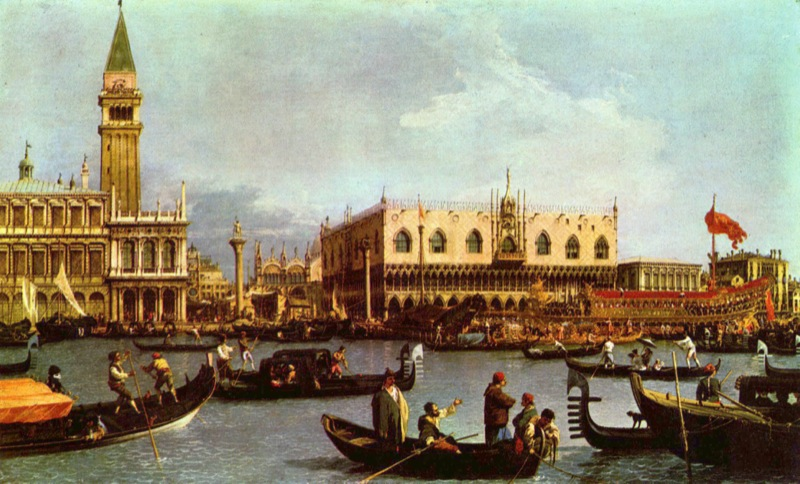
\includegraphics[width=0.9\textwidth]{pictures/canaletto}
\end{center}

\end{frame}

\begin{frame}
\frametitle{Die Aufforderung zum Duell}
\framesubtitle{Steckbrief}

\frakfamily\Large
\begin{center}
\colorbox{orange}{
\parbox{\dimexpr 0.8\linewidth - 2\fboxrule - 2\fboxsep}{
\begin{center}

Hiermit fordere ich, Antoniomaria Fior,\\
den Rechenmeister Niccol� Tartaglia\\
zum Duell heraus:.\\[2ex]

Der Heraus:geforderte m�ge sich am\\
10. Januar 1535 a.D. bei Notar Zambelli\\
in der Foscarigasse melden.
\end{center}
}
}
\end{center}
\normalfont\normalsize
\end{frame}

%\begin{frame}
%\frametitle{Die Aufforderung zum Duell}
%\framesubtitle{Steckbrief}

%\bsifamily\large
%\begin{center}
%\colorbox{orange}{
%\parbox{\dimexpr 0.8\linewidth - 2\fboxrule - 2\fboxsep}{
%\begin{center}

%Hiermit fordere ich, Antoniomaria Fier,\\
%den Rechenmeister Niccol� Tartaglia\\
%zum Duell heraus.\\[2ex]

%Der Herausgeforderte m�ge sich am\\
%10. Januar 1535 a.D. bei Notar Zambelli\\
%in der Foscarigasse melden.
%\end{center}
%}
%}
%\end{center}
%\normalfont\normalsize
%\end{frame}

\begin{frame}
\normalfont
\frametitle{Niccol� Tartaglia}
\framesubtitle{~1500 -- 1557}

\begin{columns}
\column{0.6\textwidth}
\begin{itemize}
\item urspr�nglich wohl Niccol� Fontana
\item 1512 in Brescia schwer verwundet\\
$\rightarrow$ stottert
\item arbeitet als Rechenlehrer
\item 1534 Umzug nach Venedig
\end{itemize}
\column{0.4\textwidth}
\begin{center}
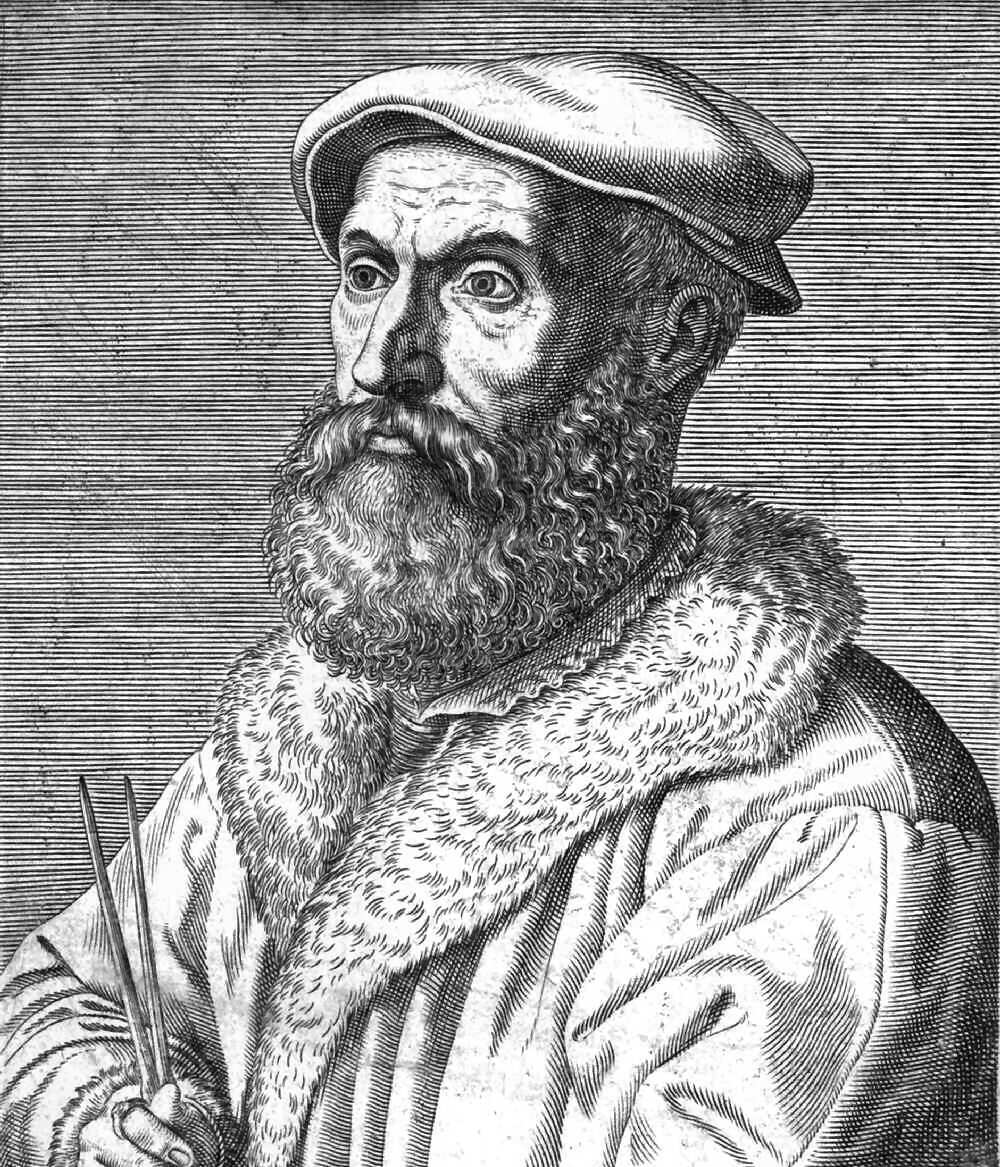
\includegraphics[width=0.9\textwidth]{pictures/tartaglia}
\end{center}
\end{columns}

\note[item]{{\bf Franzoseneinfall} in Brescia; Niccol�, damals ein kleiner Junge, �berlebt schwer verletzt. Seit diesem �berfall (Kiefer zertr�mmert) f�llt ihm das Sprechen aufgrund seiner Verletzungen schwer. Er erh�lt den �bernahmen {\bf \glqq der Stotterer\grqq}.}
\note[item]{Hilft Kaufleuten beim Berechnen von Zinsen, berechnet Brotpreise f�r die Stadt {\bf Verona}.}

\end{frame}

\begin{frame}
\frametitle{Das Duell}
\framesubtitle{Die Regeln}

\begin{itemize}
\item 30 Aufgaben f�r den Kontrahenten
\item 1 Monat Zeit
\item Sieger ist, wer mehr Aufgaben korrekt l�sen kann
\item Preis: Ehre, 1 Abendessen f�r jede nicht gel�ste Aufgabe
\end{itemize}

\note[item]{Lernende erfinden ihre eigenen Duellaufgaben}

\end{frame}

\begin{frame}
\frametitle{Mathematik zur Zeit Tartaglias}
\framesubtitle{Euklid (4 v.u.Z.), \visible<2->{Al-Chwarizmi (9. Jh.)}, \visible<3->{Fibonacci (13. Jh.)}, \visible<4->{Pacioli (15. Jh.)}}

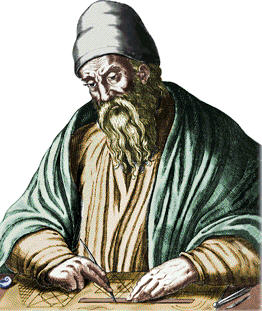
\includegraphics[width=2cm]{pictures/euklid}\hspace*{0.3\textwidth} \visible<3->{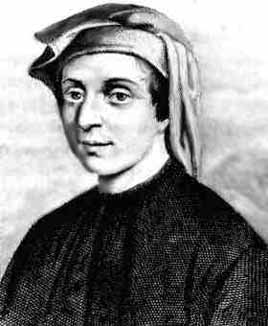
\includegraphics[width=2cm]{pictures/fibonacci}}\\[4ex]

\hspace*{0.2\textwidth} \visible<2->{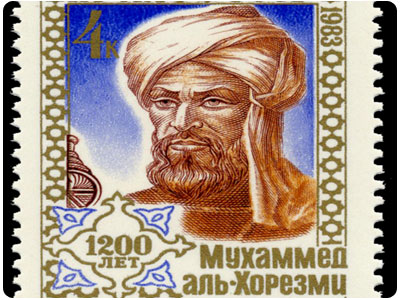
\includegraphics[width=3cm]{pictures/al-chwarizmi}}\hspace*{0.2\textwidth}  \visible<4->{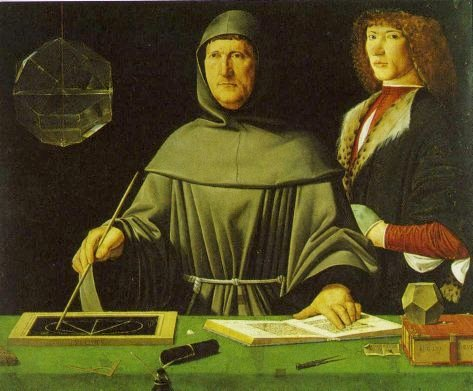
\includegraphics[width=3cm]{pictures/pacioli}}

\end{frame}

\note[item]{{\bf Euklid von Alexandria} (ca. 360 v. Chr. bis ca. 280 v. Chr.) war ein griechischer Mathematiker.

Die �berlieferten Werke umfassen s�mtliche Bereiche der antiken griechischen Mathematik: das sind die theoretischen Disziplinen \emph{Arithmetik und Geometrie} (Die Elemente, Data), \emph{Musiktheorie} (Die Teilung des Kanon), eine methodische Anleitung zur Findung von \emph{planimetrischen Probleml�sungen} von bestimmten gesicherten Ausgangspunkten aus (Porismen) sowie die \emph{physikalischen bzw. angewandten Werke} (Optik, astronomische Ph�nomene).}

\note[item]{In seinem ber�hmtesten Werk {\bf \glqq Die Elemente\grqq} (altgriechisch \glqq Anfangsgr�nde, Prinzipien, Elemente\grqq; vermutlich um 325 v. Chr. entstanden) trug er das Wissen der griechischen Mathematik seiner Zeit zusammen. Er zeigte darin die Konstruktion geometrischer Objekte, nat�rlicher Zahlen sowie bestimmter Gr�ssen und untersuchte deren Eigenschaften. Dazu benutzte er Definitionen, Postulate (nach Aristoteles Grunds�tze, die akzeptiert oder abgelehnt werden k�nnen) und Axiome (nach Aristoteles allgemeine und unbezweifelbare Grunds�tze). Viele S�tze der Elemente stammen offenbar nicht von Euklid selbst. Seine Hauptleistung besteht vielmehr in der Sammlung und einheitlichen Darstellung des mathematischen Wissens sowie der strengen Beweisf�hrung, die zum Vorbild f�r die sp�tere Mathematik wurde.}

\note[item]{Abu Dscha'far Muhammad ibn Musa al-Chwarizmi, Var. {\bf Chwarazmi}, (arabisch, * um 780; � zwischen 835 (?) und 850) war ein choresmischer Universalgelehrter, Mathematiker, Astronom und Geograph w�hrend der abbasidischen Bl�tezeit, der den gr�ssten Teil seines Lebens in Bagdad verbrachte und dort im �Haus der Weisheit� t�tig war. Von seinem Namen leitet sich der Begriff Algorithmus ab.

In seinem Werk ({\bf �ber das Rechnen mit indischen Ziffern�}, um 825) stellte al-Chwarizmi die Arbeit mit Dezimalzahlen vor und f�hrte die Ziffer Null (arab.: sifr) aus dem indischen in das arabische Zahlensystem und damit in alle modernen Zahlensysteme ein. Die lateinische Fassung dieser Schrift trug den Titel Algorismi de\dots (�Das Werk des al-gorismus �ber\dots�). Daraus entstand die Bezeichnung �Algorithmus�, mit der generell genau definierte Rechenverfahren gemeint sind. Die arabische Urfassung dieses Buches ist verlorengegangen; es blieb nur in einer lateinischen �bersetzung erhalten.}

\note[item]{Im Jahr 830 schloss er die Arbeit an dem Buch Kit'b al-muchtasar fi hisab al-dschabr wa-l-muqabala (�Rechnen durch Erg�nzung und Ausgleich�) ab. Es ist eine Zusammenstellung von Regeln und Beispielen. Sein --- f�r die damalige Zeit ungew�hnliches --- systematisch-logisches Vorgehen gab den {\bf L�sungsans�tzen linearer und quadratischer Gleichungen} eine v�llig neue Richtung, n�mlich der geometrischen Bearbeitung dieser Gleichungen, was zu einer neuen Form von Verst�ndnis f�r diese Aufgabenklasse f�hrt. Diese �bildhafte� Darstellung mathematischer Probleme macht das Thema nicht nur greifbarer, sondern f�hrt zu einer Art der Erkenntnisgewinnung, welche f�r �Laien� weitaus nachvollziehbarer ist. Die Leistung besteht also auch darin, dass er damit ein sehr effizientes mathematisches �Werkzeug� geschaffen hat.}

\note[item]{Das Buch wurde vom 12. Jahrhundert an mehrfach ins Lateinische �bersetzt; dabei wurde der Begriff {\bf �Algebra�} aus dem Titel dieses Werkes (al-`jabr) abgeleitet. Es hatte grossen Einfluss auf die Mathematik im Vorderen Orient und dann auch auf die weitere Entwicklung im Westen.}

\note[item]{{\bf Leonardo da Pisa}, auch Fibonacci genannt (* um 1180? in Pisa; � nach 1241 ebenda) war Rechenmeister in Pisa und gilt als der bedeutendste Mathematiker des Mittelalters. Bekannt sind heute vor allem die nach ihm benannten Fibonacci-Zahlen.

Leonardo war in den neunziger Jahren des 12. Jahrhunderts folglich nicht der erste Lateiner, der das Rechnen mit den neuen Ziffern erlernte, aber er erwarb in Bougie offenbar mathematische Grundlagen, die er h�her sch�tzte als alles, was er bei weiteren Studien an Handelsorten �in �gypten, Syrien, Griechenland, Sizilien und S�dfrankreich� noch erlernte. Als von ihm vergleichsweise gering, �gleichsam als Irrtum� eingesch�tzte Methoden nennt er besonders den �Algorismus�, worunter das elementare Ziffernrechnen nach Al-Chwarizmi verstanden wurde, von dem sich Leonardos eigene Mathematik eigentlich nur durch die anspruchsvollere Anwendung der Verfahren unterschied, sowie eine von ihm als �B�gen des Pythagoras� umschriebene Methode:}

\note[item]{gemeint ist das abazistische Rechnen auf dem im 10. bis 12. Jahrhundert gebr�uchlich gewesenen, zu Leonardos Zeit wieder weitgehend ausser Gebrauch gekommenen Gerbertschen Abakus, der als Erfindung des Pythagoras galt und auf dem im Unterschied zu den sp�teren mittelalterlichen Rechenbrettern mit bezifferten Rechensteinen (beziffert mit arabischen Ghubar-Ziffern 1-9) gerechnet wurde.}

\note[item]{{\bf Luca Pacioli} (* um 1445 in Borgo San Sepolcro (heute Sansepolcro), Toskana; � 1514 oder 1517 in Rom) war ein italienischer Mathematiker und Franziskaner. Bekannt ist er in den Wirtschaftswissenschaften, weil er 1494 als erster die doppelte Buchf�hrung komplett beschreibt.

Paciolis Wirkung gr�ndet sich vor allem auf sein Buch {\bf \glqq Summa de Arithmetica, Geometria, Proportioni et Proportionalit�\grqq} (1487 vollendet und 1494 gedruckt, 2. Auflage 1523), das wahrscheinlich das erste gedruckte Buch eines Mathematikers ist und entsprechend viel verwendet wurde. Es bietet wenig eigenst�ndige Ideen, aber b�ndelt das wichtigste mathematische Wissen, auf der Grundlage u.a. des Liber Abbaci des Leonardo Fibonacci, 1202, 2. A. 1228, welches die L�sungen f�r Gleichungen erster und zweiter Ordnung von Al-Chwarizmi �berliefert hatte, was aber bis zum Wiederaufgreifen durch Pacioli kaum bekannt war.}

\note[item]{Pacioli verarbeitet auch die Werke von Jordanus Nemorarius, 1236, und Johannes de Sacrobosco, 1256). Diese Kenntnisse wurden an den damaligen italienischen Abakus-Schulen f�r Kaufleute gelehrt. Das Buch enth�lt die erste geschlossene Darstellung der �Venezianischen Methode� (doppelte Buchf�hrung), wie sie zu diesem Zeitpunkt wahrscheinlich von den Venezianern und Medici verwendet wurde. Allerdings erw�hnt er zugleich die Verwendung derselben in den B�chern der Finanzbeamten Genuas und ist, entgegen vielen Meinungen, nicht der Erfinder der doppelten Buchf�hrung. Dieser ist vermutlich der aus Ragusa stammende H�ndler Benedetto Cotrugli. Das Buch wurde indes in viele Sprachen �bersetzt und von anderen Autoren kopiert, was der doppelten Buchf�hrung zu ihrem Durchbruch verhalf.}

\note[item]{\emph{Pacioli fand keine L�sung f�r Kubische Gleichungen ($x^3+mx=n \text{ oder } x^3+n=mx$) und beschliesst sein Werk mit der Behauptung, diese seien beim Stand der Wissenschaft so wenig allgemein l�sbar wie die Quadratur des Kreises; es bestehe jedoch Anlass zur Hoffnung, dass zuk�nftig L�sungen gefunden w�rden}. So war es in der Tat, auch durch diese Bemerkungen angeregt, und zwar zuerst bei den L�sungswegen, die Scipione del Ferro und Nicolo von Brescia (\glqq Tartaglia\grqq genannt) fanden. Auch diskutiert Pacioli das Teilungsproblem.}

\section{Das Ringen um die kubische Gleichung}

\begin{frame}
\frametitle{Die Aufgaben von Fior}
\framesubtitle{Ausz�ge}

\begin{itemize}
\item[5.] Zwei M�nner gr�nden eine Gesellschaft, wobei die beiden zusammen 900 Dukaten Kapital einbringen m�ssen, mit der Bedingung, dass der eine die Kubikwurzel des anderen einbringt. Ich frage, wie viel jeder in die besagte Gesellschaft einbringen muss?
\item[12.] Ein Juwelier verkauft zwei Schmuckst�cke f�r zweitausend und neunhundert Dukaten, n�mlich einen Diamanten und einen Rubin, und der Rubin wurde zur Kubikwurzel des Wertes des Diamanten verkauft. Ich frage, wie viel der Rubin wert war?
\item[22.] Es sind zwei gleichseitige Sechsecke, deren Fl�chen zusammen 27 Ellen ergeben, und das kleinere Sechseck ist die Kubikwurzel des gr�sseren. Ich frage nach der Fl�che des kleineren.
\end{itemize}

\note[item]{Der freche Fior stellt alles Aufgaben vom gleichen Typ}

\end{frame}

\begin{frame}
\frametitle{Die Aufgaben von Fior}
\framesubtitle{Algebraische �bersetzung}

\begin{itemize}
\item[5.] $$x^3+x=900$$
\item[12.] $$x^3+x=2900$$
\item[22.] $$x^3+x=27$$
\end{itemize}

\end{frame}

\begin{frame}
\frametitle{Die Aufgaben von Fior}
\framesubtitle{Algebraische �bersetzung}

\begin{alertblock}{Die Aufgaben von Fior}
Aufgaben sind alle vom Typ
$$x^3+px=q$$
\end{alertblock}

\end{frame}

\begin{frame}
\frametitle{Al-Chwarizmis Gnomon}
\framesubtitle{noch 21 Tage}

\begin{columns}
\column{0.6\textwidth}
\begin{center}
\scalebox{.9}{
\begin{tikzpicture}[line cap=round,line join=round,>=triangle 45,x=1.0cm,y=1.0cm]
\clip(-5.05,-2.15) rectangle (4.03,4.96);
\draw (-3,4)-- (-3,-1);
\draw (-3,-1)-- (2,-1);
\draw (2,4)-- (-3,4);
\draw (2,4)-- (2,-1);
\draw (-3,3)-- (2,3);
\draw (1,4)-- (1,-1);
\draw (-3,3.8) node[anchor=north west] {$5$};
\draw (1.25,-0.5) node[anchor=north west] {$5$};
\draw (-1.3,3.87) node[anchor=north west] {\colorbox{yellow}{$5x$}};
\draw (1.1,1.5) node[anchor=north west] {\colorbox{yellow}{$5x$}};
\draw (-1.3,1.58) node[anchor=north west] {\colorbox{yellow}{$x^2$}};
\draw (-3,1.47) node[anchor=north west] {$x$};
\draw (-0.96,-0.55) node[anchor=north west] {$x$};
\draw (1.1,3.9) node[anchor=north west] {\colorbox{yellow}{$5^2$}};
\end{tikzpicture}
}
\end{center}
\column{0.4\textwidth}
\begin{align*}
x^2+10x&=96\\
x^2+2\cdot 5\cdot x&=96\\
x^2+2\cdot 5\cdot x+25&=96+25\\
(x+5)^2 &= 121\\
x+5 &=11\\
x&=6
\end{align*}
\end{columns}

\end{frame}


\begin{frame}
\frametitle{Regiomontans Gnomon}
\framesubtitle{noch 17 Tage}


\begin{center}
\scalebox{.9}{
\begin{tikzpicture}[line cap=round,line join=round,>=triangle 45,x=1.0cm,y=1.0cm]
\clip(-3.38,-2.48) rectangle (5.82,1.54);
\draw (-3,-2)-- (-3,-1);
\draw (-3,-1)-- (2,-1);
\draw (-3,-2)-- (2,-2);
\draw (2,-1)-- (2,-2);
\draw (2,-1)-- (5,1);
\draw (2,-2)-- (5,0);
\draw (5,1)-- (5,0);
\draw (-3,-1)-- (0,1);
\draw (0,1)-- (5,1);
\draw (1,-1)-- (4,1);
\draw (1,-1)-- (1,-2);
\draw (-0.56,0.62)-- (4.43,0.62);
\draw (4.43,0.62)-- (4.43,-0.38);
\draw [dash pattern=on 3pt off 3pt] (4.43,-0.38)-- (3.43,-0.38);
\draw [dash pattern=on 3pt off 3pt] (3.43,0.62)-- (3.43,-0.38);
\draw [dash pattern=on 3pt off 3pt] (3.43,-0.38)-- (1,-2);
\end{tikzpicture}
}
\end{center}

\end{frame}

\begin{frame}
\frametitle{Tartaglias Gnomon}
\framesubtitle{noch 16 Tage}


\begin{center}
\scalebox{.7}{
\begin{tikzpicture}[line cap=round,line join=round,>=triangle 45,x=1.0cm,y=1.0cm]
\clip(-3.38,-6.52) rectangle (5.58,1.54);
\draw (-3,-1)-- (2,-1);
\draw (-3,-2)-- (2,-2);
\draw (2,-1)-- (5,1);
\draw (2,-2)-- (5,0);
\draw (-3,-1)-- (0,1);
\draw (0,1)-- (5,1);
\draw (1,-1)-- (4,1);
\draw (-0.56,0.63)-- (4.43,0.62);
\draw [dash pattern=on 2pt off 2pt] (3.43,-0.38)-- (1,-2);
\draw (-3,-1)-- (-3,-6);
\draw (-3,-6)-- (2,-6);
\draw (2,-6)-- (5,-4);
\draw (1,-1)-- (1,-6);
\draw (2,-1)-- (2,-6);
\draw (4.43,0.62)-- (4.43,-4.38);
\draw (5,1)-- (5,-4);
\draw [dash pattern=on 2pt off 2pt] (1,-6)-- (4,-4);
\draw [dash pattern=on 2pt off 2pt] (4,-4)-- (5,-4);
\draw [dash pattern=on 2pt off 2pt] (3.43,-4.38)-- (4.43,-4.38);
\draw [dash pattern=on 2pt off 2pt] (3.43,-4.38)-- (3.43,0.62);
\draw [dash pattern=on 2pt off 2pt] (4.43,-0.38)-- (-0.56,-0.37);
\draw [dash pattern=on 2pt off 2pt] (-3,-2)-- (-0.56,-0.37);
\draw [dash pattern=on 2pt off 2pt] (-0.56,-0.37)-- (-0.56,0.63);
\end{tikzpicture}
}
\end{center}

\end{frame}

\begin{frame}
\frametitle{Tartaglias Gnomon}
\framesubtitle{noch 8 Tage}

\begin{columns}
\column{0.6\textwidth}
\begin{center}
\scalebox{.6}{
\definecolor{qqffff}{rgb}{0,1,1}%cyan
\definecolor{ffqqqq}{rgb}{1,0,0}%rot
\definecolor{ffqqff}{rgb}{1,0,1}
\definecolor{qqqqff}{rgb}{0,0,1}
\definecolor{qqffqq}{rgb}{0,1,0}%gr�n
\begin{tikzpicture}[line cap=round,line join=round,>=triangle 45,x=1.0cm,y=1.0cm]
\clip(-3.38,-6.48) rectangle (5.8,1.54);
\draw [line width=1.6pt,dash pattern=on 2pt off 2pt,color=qqffff] (3.52,-4.29)-- (3.95,-4);%cyan
\draw [line width=1.6pt,dash pattern=on 2pt off 2pt,color=qqffff] (4,-4)-- (4,-0.38);
\draw [line width=1.6pt,dash pattern=on 2pt off 2pt,color=qqffff] (-0.52,-0.28)-- (-0.52,0.72);
\draw [line width=1.6pt,dash pattern=on 2pt off 2pt,color=qqffff] (3.49,-4.29)-- (3.49,0.72);
\draw [line width=1.6pt,color=qqffff] (-0.52,0.72)-- (0.05,1.05);
\draw [line width=1.6pt,color=qqffff] (0.05,1.05)-- (4,1.05);
\draw [line width=1.6pt,color=qqffff] (4,1.05)-- (3.46,0.72);
\draw [line width=1.6pt,color=qqffff] (3.46,0.72)-- (-0.52,0.72);
\visible<2>{\draw [line width=1.6pt,dash pattern=on 2pt off 2pt,color=qqffff] (4,-0.38)-- (4,1.05);
\draw [line width=1.6pt,dash pattern=on 2pt off 2pt,color=qqffff] (-0.52,-4.29)-- (-0.52,0.72);
\draw [line width=1.6pt,dash pattern=on 2pt off 2pt,color=qqffff]  (-0.52,-4.29)-- (3.52,-4.29);}
\visible<1,3->{\draw [line width=1.6pt,color=ffqqqq] (3.53,0.72)-- (4.05,1.05);%rot
\draw [line width=1.6pt,color=ffqqqq] (4.05,1.05)-- (5.05,1.05);
\draw [line width=1.6pt,color=ffqqqq] (5.05,1.05)-- (4.53,0.72);
\draw [line width=1.6pt,color=ffqqqq] (5.05,1.05)-- (5.05,0.05);
\draw [line width=1.6pt,color=ffqqqq] (5.05,0.05)-- (4.53,-0.28);
\draw [line width=1.6pt,color=ffqqqq] (3.53,0.72)-- (4.53,0.72);
\draw [line width=1.6pt,color=ffqqqq] (4.53,0.72)-- (4.53,-0.28);
\draw [line width=1.6pt,dash pattern=on 2pt off 2pt,color=ffqqqq] (3.53,0.72)-- (3.53,-0.28);
\draw [line width=1.6pt,dash pattern=on 2pt off 2pt,color=ffqqqq] (3.53,-0.28)-- (4.53,-0.28);}
\visible<1,4->{\draw [line width=2pt,color=qqffqq] (-3,-6)-- (1,-6);%gr�n
\draw [line width=2pt,color=qqffqq] (-3,-6)-- (-3,-2);%
\draw [line width=2pt,color=qqffqq] (-3,-2)-- (1,-2);%
\draw [line width=2pt,color=qqffqq] (1,-2)-- (1,-6);%
\draw [line width=2pt,color=qqffqq] (-3,-2)-- (-0.56,-0.38);
\draw [line width=2pt,color=qqffqq] (-0.56,-0.38)-- (3.43,-0.38);%
\draw [line width=2pt,color=qqffqq] (1,-2)-- (3.43,-0.38);%
\draw [line width=2pt,color=qqffqq] (1,-6)-- (3.43,-4.38);%
\draw [line width=2pt,color=qqffqq] (3.43,-4.38)-- (3.43,-0.38);}

\visible<3>{\draw [ForestGreen, fill=green] (-3,-6) -- (-3,-2) -- (1,-2) -- (1,-6) -- (-3,-6);
\draw [ForestGreen, fill=green] (1,-6) -- (1,-2) -- (3.43,-0.38) -- (3.43,-4.38) -- (1,-6);
\draw [ForestGreen, fill=green] (-0.56,-0.38) -- (-3,-2) -- (1,-2) -- (3.43,-0.38) -- (-0.56,-0.38);}

\draw [line width=2pt,dash pattern=on 1pt off 4pt,color=qqqqff] (1.05,-6)-- (4.05,-4);%blau
\draw [line width=1.6pt,dash pattern=on 2pt off 2pt,color=qqqqff] (1.05,-2)-- (3.53,-0.38);
\draw [line width=1.6pt,color=qqqqff] (1.05,-2)-- (1.05,-6);
\draw [line width=1.6pt,color=qqqqff] (1.05,-6)-- (2.05,-6);
\draw [line width=1.6pt,color=qqqqff] (2.05,-6)-- (5.05,-4);
\draw [line width=1.6pt,dash pattern=on 2pt off 2pt,color=qqqqff] (4.05,-4)-- (5.05,-4);
\draw [line width=1.6pt,color=qqqqff] (5.05,-4)-- (5.05,0);
\draw [line width=1.6pt,color=qqqqff] (5.05,0)-- (2.05,-2);
\draw [line width=1.6pt,color=qqqqff] (1.05,-2)-- (2.05,-2);
\draw [line width=1.6pt,color=qqqqff] (2.05,-2)-- (2.05,-6);
\visible<2>{\draw [line width=1.6pt,dash pattern=on 2pt off 2pt,color=qqqqff] (4.05,0)-- (5.05,0);
\draw [line width=1.6pt,dash pattern=on 2pt off 2pt,color=qqqqff] (3.53,-0.38)-- (4.05,0);
\draw [line width=1.6pt,dash pattern=on 2pt off 2pt,color=qqqqff] (4.05,-4)-- (4.05,0);}
\draw [line width=1.6pt,color=ffqqff] (-3,-0.95)-- (2.05,-0.95);%magenta
\draw [line width=1.6pt,color=ffqqff] (2.05,-0.95)-- (4.48,0.68);
\draw [line width=1.6pt,color=ffqqff] (4.48,0.68)-- (-0.56,0.68);
\draw [line width=1.6pt,color=ffqqff] (-0.56,0.68)-- (-3,-0.95);
\draw [line width=1.6pt,color=ffqqff] (-3,-1.95)-- (2.05,-1.95);
\draw [line width=1.6pt,color=ffqqff] (2.05,-1.95)-- (4.48,-0.33);
\draw [line width=1.6pt,dash pattern=on 2pt off 2pt,color=ffqqff] (4.48,-0.33)-- (-0.56,-0.33);
\draw [line width=1.6pt,dash pattern=on 2pt off 2pt,color=ffqqff] (-0.56,-0.33)-- (-3,-1.95);
\draw [line width=1.6pt,color=ffqqff] (-3,-0.95)-- (-3,-1.95);
\draw [line width=1.6pt,dash pattern=on 2pt off 2pt,color=ffqqff] (-0.56,0.68)-- (-0.56,-0.33);
\draw [line width=1.6pt,color=ffqqff] (4.48,0.68)-- (4.48,-0.33);
\draw [line width=1.6pt,color=ffqqff] (2.05,-0.95)-- (2.05,-1.95);
\draw (5.1,0.8) node[anchor=north west] {$x$};
\draw (5.1,-1.5) node[anchor=north west] {$y$};
\draw (3.76,-4.9) node[anchor=north west] {$l$};
\end{tikzpicture}
}
\end{center}

\column{0.4\textwidth}
Wir haben $x^3+px=q.$

\visible<2->{Setze $$px=3lyx, y=\dfrac{p}{3l}.$$}

\visible<3->{Es gilt auch $l^3-y^3=q.$}

\visible<4->{Damit
\begin{align*}
l^3-\left(\frac{p}{3l}\right)^3 &=q\\
l^6-ql^3-\left(\frac{p}{3}\right)^3 &=0\\
u^2-qu-\left(\frac{p}{3}\right)^3 &=0
\end{align*}}

\end{columns}

\end{frame}

\begin{frame}
\frametitle{Tartaglias Gnomon}
\framesubtitle{noch 8 Tage}

\begin{columns}

\column{0.4\textwidth}
Mit Zauberformel:
$$u=\frac{q}{2}\pm\sqrt{\left(\frac{q}{2}\right)^2+\left(\frac{p}{3}\right)^3}.$$
Wegen der Geometrie
$$u=\frac{q}{2}+\sqrt{\left(\frac{q}{2}\right)^2+\left(\frac{p}{3}\right)^3}.$$
Wegen $u=l^3$ hat man
$$l=\sqrt[3]{\frac{q}{2}+\sqrt{\left(\frac{q}{2}\right)^2+\left(\frac{p}{3}\right)^3}}.$$

\column{0.6\textwidth}
\begin{center}
\scalebox{.6}{
\definecolor{qqffff}{rgb}{0,1,1}%cyan
\definecolor{ffqqqq}{rgb}{1,0,0}%rot
\definecolor{ffqqff}{rgb}{1,0,1}
\definecolor{qqqqff}{rgb}{0,0,1}
\definecolor{qqffqq}{rgb}{0,1,0}%gr�n
\begin{tikzpicture}[line cap=round,line join=round,>=triangle 45,x=1.0cm,y=1.0cm]
\clip(-3.38,-6.48) rectangle (5.8,1.54);
\draw [line width=1.6pt,dash pattern=on 2pt off 2pt,color=qqffff] (3.52,-4.29)-- (3.95,-4);%cyan
\draw [line width=1.6pt,dash pattern=on 2pt off 2pt,color=qqffff] (3.95,-4)-- (3.95,-0.38);
\draw [line width=1.6pt,dash pattern=on 2pt off 2pt,color=qqffff] (-0.52,-0.28)-- (-0.52,0.72);
\draw [line width=1.6pt,dash pattern=on 2pt off 2pt,color=qqffff] (3.49,-4.29)-- (3.49,0.72);
\draw [line width=1.6pt,color=qqffff] (-0.52,0.72)-- (0.05,1.05);
\draw [line width=1.6pt,color=qqffff] (0.05,1.05)-- (4,1.05);
\draw [line width=1.6pt,color=qqffff] (4,1.05)-- (3.46,0.72);
\draw [line width=1.6pt,color=qqffff] (3.46,0.72)-- (-0.52,0.72);
\draw [line width=1.6pt,color=ffqqqq] (3.53,0.72)-- (4.05,1.05);%rot
\draw [line width=1.6pt,color=ffqqqq] (4.05,1.05)-- (5.05,1.05);
\draw [line width=1.6pt,color=ffqqqq] (5.05,1.05)-- (4.53,0.72);
\draw [line width=1.6pt,color=ffqqqq] (5.05,1.05)-- (5.05,0.05);
\draw [line width=1.6pt,color=ffqqqq] (5.05,0.05)-- (4.53,-0.28);
\draw [line width=1.6pt,color=ffqqqq] (3.53,0.72)-- (4.53,0.72);
\draw [line width=1.6pt,color=ffqqqq] (4.53,0.72)-- (4.53,-0.28);
\draw [line width=1.6pt,dash pattern=on 2pt off 2pt,color=ffqqqq] (3.53,0.72)-- (3.53,-0.28);
\draw [line width=1.6pt,dash pattern=on 2pt off 2pt,color=ffqqqq] (3.53,-0.28)-- (4.53,-0.28);
\draw [line width=2pt,color=qqffqq] (-3,-6)-- (1,-6);%gr�n
\draw [line width=2pt,color=qqffqq] (-3,-6)-- (-3,-2);
\draw [line width=2pt,color=qqffqq] (-3,-2)-- (1,-2);
\draw [line width=2pt,color=qqffqq] (1,-2)-- (1,-6);
\draw [line width=2pt,color=qqffqq] (-3,-2)-- (-0.56,-0.38);
\draw [line width=2pt,color=qqffqq] (-0.56,-0.38)-- (3.43,-0.38);
\draw [line width=2pt,color=qqffqq] (1,-2)-- (3.43,-0.38);
\draw [line width=2pt,color=qqffqq] (1,-6)-- (3.43,-4.38);
\draw [line width=2pt,color=qqffqq] (3.43,-4.38)-- (3.43,-0.38);
\draw [line width=2pt,dash pattern=on 2pt off 2pt,color=qqqqff] (1.05,-6)-- (4.05,-4);%blau
\draw [line width=1.6pt,dash pattern=on 2pt off 2pt,color=qqqqff] (1.05,-2)-- (3.53,-0.38);
\draw [line width=1.6pt,color=qqqqff] (1.05,-2)-- (1.05,-6);
\draw [line width=1.6pt,color=qqqqff] (1.05,-6)-- (2.05,-6);
\draw [line width=1.6pt,color=qqqqff] (2.05,-6)-- (5.05,-4);
\draw [line width=1.6pt,dash pattern=on 2pt off 2pt,color=qqqqff] (4.05,-4)-- (5.05,-4);
\draw [line width=1.6pt,color=qqqqff] (5.05,-4)-- (5.05,0);
\draw [line width=1.6pt,color=qqqqff] (5.05,0)-- (2.05,-2);
\draw [line width=1.6pt,color=qqqqff] (1.05,-2)-- (2.05,-2);
\draw [line width=1.6pt,color=qqqqff] (2.05,-2)-- (2.05,-6);
\draw [line width=1.6pt,color=ffqqff] (-3,-0.95)-- (2.05,-0.95);%magenta
\draw [line width=1.6pt,color=ffqqff] (2.05,-0.95)-- (4.48,0.68);
\draw [line width=1.6pt,color=ffqqff] (4.48,0.68)-- (-0.56,0.68);
\draw [line width=1.6pt,color=ffqqff] (-0.56,0.68)-- (-3,-0.95);
\draw [line width=1.6pt,color=ffqqff] (-3,-1.95)-- (2.05,-1.95);
\draw [line width=1.6pt,color=ffqqff] (2.05,-1.95)-- (4.48,-0.33);
\draw [line width=1.6pt,dash pattern=on 2pt off 2pt,color=ffqqff] (4.48,-0.33)-- (-0.56,-0.33);
\draw [line width=1.6pt,dash pattern=on 2pt off 2pt,color=ffqqff] (-0.56,-0.33)-- (-3,-1.95);
\draw [line width=1.6pt,color=ffqqff] (-3,-0.95)-- (-3,-1.95);
\draw [line width=1.6pt,dash pattern=on 2pt off 2pt,color=ffqqff] (-0.56,0.68)-- (-0.56,-0.33);
\draw [line width=1.6pt,color=ffqqff] (4.48,0.68)-- (4.48,-0.33);
\draw [line width=1.6pt,color=ffqqff] (2.05,-0.95)-- (2.05,-1.95);
\draw (5.1,0.8) node[anchor=north west] {$x$};
\draw (5.1,-1.5) node[anchor=north west] {$y$};
\draw (3.76,-4.9) node[anchor=north west] {$l$};
\end{tikzpicture}
}
\end{center}

\end{columns}

\end{frame}

\begin{frame}
\frametitle{Tartaglias Gnomon}
\framesubtitle{noch 7 Tage}

Einsetzen von $$l=\sqrt[3]{\frac{q}{2}+\sqrt{\left(\frac{q}{2}\right)^2+\left(\frac{p}{3}\right)^3}}$$ in $y^3=l^3-q$ ergibt
$$y=-\sqrt[3]{\frac{q}{2}-\sqrt{\left(\frac{q}{2}\right)^2+\left(\frac{p}{3}\right)^3}}.$$

Aus $x=l-y$ folgt

\begin{exampleblock}{Formel von Cardano}
$$x=\sqrt[3]{\frac{q}{2}+\sqrt{\left(\frac{q}{2}\right)^2+\left(\frac{p}{3}\right)^3}}+\sqrt[3]{\frac{q}{2}-\sqrt{\left(\frac{q}{2}\right)^2+\left(\frac{p}{3}\right)^3}}.$$
\end{exampleblock}

\note[item]{Damit kann Tartaglia nun alle Gleichungen von Fior l�sen, wenn er die Kubikwurzel ziehen kann; dazu in K�rze.}

\end{frame}

\section{Die allgemeine kubische Gleichung}

\begin{frame}
\frametitle{Allgemeine kubische Gleichung}
\framesubtitle{Freude herrscht}

$$x^3+bx^2+cx+d=0\vspace*{4ex}$$

\visible<2->{Substitution mit $x=y-\frac{b}{3}$} \visible<3->{ergibt eine kubische Gleichung \glqq fior'schen\grqq Typs:
$$y^3-\frac{b^2-3c}{3}y+\left(\frac{2b^3}{27}-\frac{bc}{3}+d\right)=0.$$}

\end{frame}

\section{Ziehen von Kubikwurzeln}

\begin{frame}
\frametitle{Anwendung der Formel}
\framesubtitle{Ziehen von Kubikwurzeln?}

$$x^3+2x=12$$

Cardano sagt:

$$x=\sqrt[3]{6+\frac{14}{3}\sqrt{\frac{5}{3}}}+\sqrt[3]{6-\frac{14}{3}\sqrt{\frac{5}{3}}}$$

\note[item]{Diese Gleichung hat offensichtlich L�sung $x=2$. Die Cardanische Formel liefert aber ein erschreckendes Ergebnis.}
\note[item]{Ist dieser Ausdruck gleich 2? Wie k�nnen Kubikwurzeln gezogen werden?}

\end{frame}

\begin{frame}
\frametitle{Berechnung von $\sqrt[3]{\sqrt{108}+10}$}
\framesubtitle{Zitat von Tartaglia}

\small
\dots man muss die besagte 10 so in zwei Teile zerlegen, dass der eine von diesen eine Kubikzahl ist und der andere in drei gleiche Teile ohne Br�che geteilt werden kann, und um sie zu finden, subtrahiere ich von der besagten 10 jede von den in der besagten 10 enthaltenen Kubikzahlen, das sind 1 und 8, und schaue, welche von ihnen mir einen Rest gibt, der (wie gesagt) in drei gleiche Teile teilbar ist, und wir werden finden, dass es die 1 ist und nicht die 8. Nun sage ich, dass die Kubikwurzel aus 1, welche ebenfalls 1 ist, der kleinere Teil der besagten binomischen Kubikwurzel ist, und der andere Teil ist die Quadratwurzel aus dem Ergebnis, das herauskommt, wenn man den dritten Teil des obengenannten Restes durch den besagten kleineren Teil dividiert, das heisst, wenn man die besagte Kubikzahl 1 von 10 subtrahiert hat, bleibt 9, von welcher 9 man ihren dritten Teil nimmt, welcher 3 ist, und diesen dividieren wir durch die Kubikwurzel aus unserer Kubikzahl 1, welche ebenfalls 1 ist; aus der besagten Division wird sich ebenfalls 3 ergeben, und die Quadratwurzel aus 3 wird der gr�ssere Teil unseres Wurzelbinoms sein, das heisst, die Kubikwurzel aus $\sqrt{108}+10$ wird gleich $\sqrt{3}+1$ sein, qed.

\end{frame}
\normalsize

\begin{frame}
\frametitle{Berechnung von Kubikwurzeln}
\framesubtitle{N�herungsverfahren}

Die Kubikwurzel $\sqrt[3]{a}$ ist L�sung der Gleichung $x^3=a$ und damit eine Nullstelle des Graphen der Funktion
$$f(x)=x^3-a.$$

\begin{itemize}
\item Regula Falsi
\item Bisektionsverfahren
\item Sekantenverfahren
\item Newtonverfahren
\end{itemize}

\end{frame}

\note[item]{Das Regula-falsi-Verfahren startet mit zwei Stellen (in der N�he der Nullstelle)  $a_0$ und $b_0$, deren Funktionsauswertungen $f(a_0)$, $f(b_0)$ unterschiedliche Vorzeichen haben. In dem Intervall $[a,b]$ befindet sich somit nach dem Zwischenwertsatz (f�r stetiges $f$) eine Nullstelle. Nun verkleinert man in mehreren Iterationsschritten das Intervall und bekommt so eine immer genauere N�herung f�r die Nullstelle.}

\note[item]{Die Bisektion, fortgesetzte Bisektion oder auch Intervallhalbierungsverfahren genannt, ist ein Verfahren der Mathematik und der Informatik. Durch sie wird eine konvergente Folge von Intervallschachtelungen erzeugt. Das Wort setzt sich zusammen aus Bi �Zwei� und Sektion �Schnitt�. Es steht also f�r Zwei-Teilung.
Grunds�tzlich finden Bisektionsverfahren immer dann Anwendung, wenn ein Problem gel�st werden kann, indem es in zwei etwa gleich grosse Teilprobleme zerlegt wird, die dann einzeln f�r sich behandelt werden k�nnen.}

\note[item]{Bei dem Sekantenverfahren handelt es sich um ein schon seit dem Mittelalter bekanntes numerisches Verfahren zur n�herungsweisen L�sung einer Gleichung des Typs $f(x)=0$. Es entspricht einer Vereinfachung des Newton-Verfahrens, da nicht die Ableitung der Funktion berechnet werden muss.}

\note[item]{Das Newton-Verfahren, auch Newton-Raphson-Verfahren, (benannt nach Sir Isaac Newton 1669 und Joseph Raphson 1690) ist in der Mathematik ein Standardverfahren zur numerischen L�sung von nichtlinearen Gleichungen und Gleichungssystemen. Im Falle einer Gleichung mit einer Variablen lassen sich zu einer gegebenen stetig differenzierbaren Funktion $f:\mR\longrightarrow\mR$ N�herungswerte zu L�sungen der Gleichung $f(x)=0$, d.h. N�herungen der Nullstellen dieser Funktion finden. Die grundlegende Idee dieses Verfahrens ist, die Funktion in einem Ausgangspunkt zu linearisieren, d. h. ihre Tangente zu bestimmen, und die Nullstelle der Tangente als verbesserte N�herung der Nullstelle der Funktion zu verwenden. Die erhaltene N�herung dient als Ausgangspunkt f�r einen weiteren Verbesserungsschritt. Diese Iteration erfolgt, bis die �nderung in der N�herungsl�sung eine festgesetzte Schranke unterschritten hat.}

\note[item]{Das Iterationsverfahren konvergiert im g�nstigsten Fall asymptotisch mit quadratischer Konvergenzordnung, die Zahl der korrekten Dezimalstellen verdoppelt sich dann in jedem Schritt.
Formal ausgedr�ckt wird die folgende Vorschrift wiederholt, bis eine hinreichende Genauigkeit erzielt wurde: $$x_{n+1}=x_n-\frac{f(x_n)}{f'(x_n)}.$$}

\section{Bombellis \glqq wilder Gedanke\grqq}

\begin{frame}
\frametitle{Bombellis wilder Gedanke}
\framesubtitle{Entstehung}

\begin{block}{Vor�berlegung}
Jede kubische Gleichung des \glqq Fior'schen Typs\grqq\ kann in die Form
$$x^3=mx+b$$
gebracht werden. Graphisch f�hrt diese Gleichung auf ein Schnittproblem.
\end{block}

\end{frame}

\begin{frame}
\frametitle{Bombellis wilder Gedanke}
\framesubtitle{Illustration}

\begin{columns}
\column{0.6\textwidth}

\begin{center}
\scalebox{0.6}{
\definecolor{ffqqff}{rgb}{1,0,1}
\definecolor{qqffqq}{rgb}{0,1,0}
\definecolor{qqqqff}{rgb}{0,0,1}
\definecolor{ffqqqq}{rgb}{1,0,0}
\begin{tikzpicture}[line cap=round,line join=round,>=triangle 45,x=1.0cm,y=1.0cm]
\draw[->,color=black] (-4,0) -- (4,0);
\foreach \x in {-4,-3,-2,-1,1,2,3}
\draw[shift={(\x,0)},color=black] (0pt,2pt) -- (0pt,-2pt) node[below] {\footnotesize $\x$};
\draw[color=black] (3.75,0.09) node [anchor=south west] { x};
\draw[->,color=black] (0,-5) -- (0,4);
\foreach \y in {-4,-3,-2,-1,1,2,3}
\draw[shift={(0,\y)},color=black] (2pt,0pt) -- (-2pt,0pt) node[left] {\footnotesize $\y$};
\draw[color=black] (0.07,3.54) node [anchor=west] { y};
\draw[color=black] (0pt,-10pt) node[right] {\footnotesize $0$};
\clip(-4,-5) rectangle (4,4);
\draw[line width=1.2pt,color=ffqqqq, smooth,samples=100,domain=-4.0:4.0] plot(\x,{(\x)^3});
\draw[line width=1.2pt,color=qqqqff, smooth,samples=100,domain=-4.0:3.6] plot(\x,{0-0.5*(\x)+2});
\draw[line width=1.2pt,color=qqffqq, smooth,samples=100,domain=-4.0:4.0] plot(\x,{1.75*(\x)});
\draw[line width=1.2pt,color=ffqqff, smooth,samples=100,domain=-4.0:4.0] plot(\x,{1.5*(\x)-1.25});
\end{tikzpicture}
}
\end{center}

\column{0.4\textwidth}
Es gibt immer einen Schnittpunkt!

Also hat eine kubische Gleichung immer eine (reelle) L�sung!

\end{columns}

\end{frame}

\begin{frame}
\frametitle{Rafael Bombelli}
\framesubtitle{L'Algebra, 1572}

$$x^3=15x+4$$

\begin{alertblock}<2->{Cardano liefert}
$$x=\sqrt[3]{2+\sqrt{-121}}+\sqrt[3]{2-\sqrt{-121}}$$\\[2ex]
\end{alertblock}
\ \\[2ex]

\visible<3->{$\Rightarrow x=\sqrt[3]{2+11\cdot\sqrt{-1}}+\sqrt[3]{2-11\cdot\sqrt{-1}}$\\[2ex]}

\visible<4->{Bombelli vermutet $\sqrt[3]{2+11\cdot\sqrt{-1}}=2+n\cdot\sqrt{-1}$.}

\note[item]{Diese Gleichung hat offensichtlich die L�sung $x=4$.}

\note[item]{Bombellis wilder Gedanke ist die Einf�hrung einer Zahl $i$, deren Quadrat gleich $-1$ ist.}

\note[item]{Bombellis Vermutung f�hrt ihn via $x=\sqrt[3]{2+11i}+\sqrt[3]{2-11i}=(2+i)+(2-i)$ zur L�sung $x=4$; Rechnung mit Komplexen Zahlen!}

\end{frame}
\end{document}
